
\begin{figure}
	\centering
	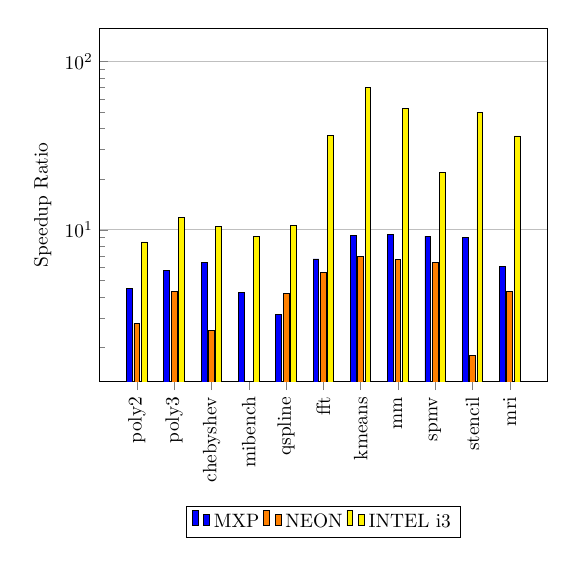
\begin{tikzpicture}[scale=0.7]
	\begin{semilogyaxis}[
	width  = 0.8*\textwidth,
	height = 8cm,
	xtick pos=left,
	ytick pos=left,
	%	major x tick style = transparent,
	x tick label style={rotate=90, anchor=east, align=right,text width=2cm},
	bar width=3pt,
	ymajorgrids = true,
	ylabel = {Speedup Ratio},
	symbolic x coords={poly2,poly3,chebyshev,mibench,qspline,fft,kmeans,mm,spmv,stencil,mri},
	xtick = data,
%	nodes near coords,
%	ybar,
%	every node near coord/.append style={rotate=90, anchor=west,font=\tiny, xshift=0.25cm},
	%	nodes near coords,
	%	ybar,
	%	every node near coord/.append style={rotate=90, anchor=west,font=\scriptsize},
	scaled y ticks = false,
	enlarge y limits={upper,value=0.2},
	%test
	%	enlarge x limits=0.25,
	ybar=2*\pgflinewidth,
	legend cell align=left,
	legend style={
		at={(.5,-0.35)},
		anchor=north,
		legend columns=-1
		column sep=0.5ex
	}
	]
	\addplot[draw=black,fill=blue]
	coordinates {(poly2,4.49) (poly3,5.709) (chebyshev,6.386) (mibench,4.22) (qspline,3.13) (fft,6.71) (kmeans,9.26) (mm,9.400) (spmv,9.1737) (stencil,9.0538) (mri,6.059) };
	
	\addplot[draw=black,fill=orange]
	coordinates	{(poly2,2.775 ) (poly3,4.32) (chebyshev,2.51) (mibench,1.25) (qspline,4.17) (fft,5.597) (kmeans,6.983) (mm,6.641) (spmv,6.4098) (stencil,1.784) (mri,4.326) };
	
	\addplot[draw=black,fill=yellow]
	coordinates	{(poly2,8.469 ) (poly3,11.834) (chebyshev,10.47) (mibench,9.122) (qspline,10.57) (fft,36.55) (kmeans,70.54) (mm,52.39) (spmv,21.96) (stencil,50) (mri,36.098) };
	
	\legend{MXP,NEON,INTEL i3}
	\end{semilogyaxis}	
	\end{tikzpicture}
	\caption{Byte level Speedup Analysis w.r.t ARMv7 for  different benchmarks.}
	\label{speedup:1}
\end{figure}



%
%
%\pgfplotsset{
%	axis background/.style={fill=none},
%	tick style=black,
%	tick label style=black,
%	grid=both,
%	xtick pos=left,
%	ytick pos=left,
%	tick style={
%		major grid style={style=white,line width=1pt},minor grid style=white,
%		tick align=outside,
%	},
%	minor tick num=4,
%}
%
%
%\begin{figure*}[!t]
%	\centering
%	\pgfplotstableread{
%		0   4.49	 2.77	8.47	   
%		1   5.70     4.32   11.83	
%		2   6.39     2.51   10.47	
%		3   4.22     1.25   9.12    
%		4   3.13     4.17   10.57     
%		5   6.71     5.59   36.55     
%		6   9.26	 6.98	70.54	
%		7   9.40	 6.64	52.39	
%		8   9.17	 6.40	21.96		
%		9   9.05	 1.7	50.00   
%		10  6.06	 4.32	36.09			
%	}\dataset
%	\begin{tikzpicture}[scale=0.75]
%	\centering
%	\begin{axis}[
%	unbounded coords=discard,
%	log basis x=10,
%	log ticks with fixed point,
%	ybar=0pt,
%	%enlarge x limits=0.05,
%	width=25cm,
%	x = 1.8cm,
%	height=8cm,
%	ymin=0,
%	ymax=80,        
%	ylabel={Speedup Ratio},
%	grid style={dotted,gray},
%	ymajorgrids=true,
%	nodes near coords,    
%	xtick=data,
%	bar width = 0.15,
%	xticklabels = {
%		\strut poly2,
%		\strut poly3,
%		\strut chebyshev,
%		\strut mibench,
%		\strut qspline,
%		\strut fft,
%		\strut kmeans,
%		\strut mm,
%		\strut spmv,
%		\strut stencil,
%		\strut
%		mri,                               
%	},
%	x tick label style={rotate=45, anchor=north east, inner sep=0mm},
%	major x tick style = {opacity=0},
%	minor x tick num = 1,
%	minor tick length=1ex,
%	every node near coord/.append style={
%		anchor=west,
%		rotate=90,
%		font=\tiny
%	},
%	]
%	\addplot[draw=black,fill=blue!90, draw opacity=1] table[x index=0,y index=1] \dataset;\label{MXP} %ano de 2013-2014
%	\addplot[draw=black,fill=green!90, draw opacity=1] table[x index=0,y index=2] \dataset;\label{NEON} %ano de 2012-2013
%	\addplot[draw=black,fill=BLACK!90, draw opacity=1] table[x index=0,y index=3] \dataset;\label{INTEL i3} %ano de 2012-2013
%%	\addplot[draw=black,fill=black!90, draw opacity=1] table[x index=0,y index=4] \dataset;\label{Intel-i3} %ano de 2012-2013
%	\end{axis}
%	\node [draw,fill=white] at (rel axis cs: 0.55,-0.40) {\shortstack[l]{
%			\ref{MXP} MXP \ref{NEON} NEON \ref{Intel-i3} Intel-i3}};
%	
%	\end{tikzpicture}
%	\caption{Byte level Speedup Analysis w.r.t ARMv7 for  different benchmarks}
%	\label{speedup:1}
%	
%\end{figure*}